\block{\strut 2. Molecular dynamics (MD)} {
        
    \vspace{0.4cm}

    \begin{center}
        \begin{tikzpicture}
            % Image 1 (nœud "image1")
            \node[anchor=west, inner sep=0] (image1) at (0,0) {
                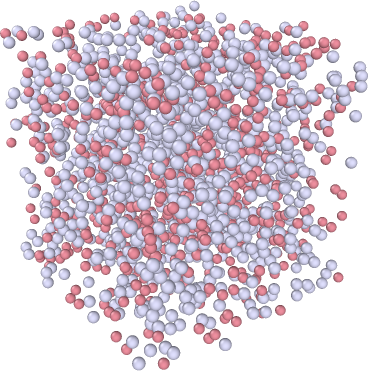
\includegraphics[width=0.2\linewidth]{Figure/MD/md_init.png}
            };

            % Image 2 (nœud "image2") à droite de l'image 1
            \node[anchor=west, inner sep=0, xshift=0.3\linewidth] (image2) at (0,0) {
               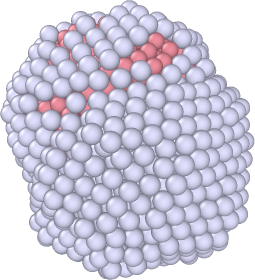
\includegraphics[width=0.18\linewidth]{Figure/MD/md_final.png}
            };

            % Légendes sous les images (optionnel)
            \node[anchor=north, align=center] at (image1.south) {\small{Initial configuration}};
            \node[anchor=north, align=center] at (image2.south) {\small{Final configuration}};

            % Flèche entre les deux images
            \draw[->, thick] (image1.east) -- (image2.west);
        \end{tikzpicture}
    \end{center}



    \textbf{\underline{Simulation protocol}}

    \vspace{0.4cm}

    \begin{itemize}
        
        \item \textbf{Number of atoms:} 10 to 5000 ;
    
        \vspace{0.25cm}
    
        \item \textbf{Simulation time:} 0.5 to 5 ns ;
            
        \vspace{0.25cm}
    
        \item \textbf{Composition:} 0\% to 100\% \textcolor{colorAg}{\textbf{Ag}} atoms, the remainder being \textcolor{colorCo}{\textbf{Co}} ;

        \vspace{0.25cm}

        \item \textbf{Initial temperature:} 1500 to 2500 K ;

        \vspace{0.25cm}

        \item \textbf{Final temperature:} 300 K ;

        \vspace{0.25cm}

        \item \textbf{Canonical ensemble:} Nos\'e--Hoover thermostat with a linear temperature decrease
                
        \vspace{0.5cm}
            
        \begin{equation}
            T(t) = \frac{T_{\text{final}} - T_\text{initial}}{t_{\text{final}}}t + T_\text{initial}
        \end{equation}            

        \vspace{1cm}

        \item \textbf{Interatomic potential:} \textbf{TBSMA} (Tight-Binding Second Moment Approximation)~[1]
                
        \vspace{0.5cm}
            
        \begin{equation}
            \mathcal{U} = \sum^N_{i=1} \left[\sum_{j\ne i}^NAe^{-p(r_{ij}/r_0 - 1)} -\sqrt{\sum_{j\ne i}^N\xi^2e^{-2q(r_{ij}/r_0 - 1)}}~\right]
        \end{equation}
    \end{itemize}

}
